%mainfile: ../master.tex
\subsection{The Iteration Problem}

The actor model makes it possible to create continuous simulations in the language, with a good abstraction for simulations and models in general. Unfortunately, the actor model does not support discrete simulations as well. When trying to implement a discrete simulation solely with actors, a problem arises that needs to be addressed.

The problem is, that there is no way to tell whether a group of actors has completed their work or not. This is important since the programmer must to be able to implement iteration steps if he or she is to create discrete simulations. The programmer has to be able to find out when one step has ended to update the state of the whole system and start a new iteration. Due to the concurrent nature of the actor model, an unfortunate variant of race conditions arise.

The problem is that there is no way for the programmer in the language to tell whether a group of actors has stopped working or not. This is important since the user must to be able to implement iteration steps if the programmer is to create discrete simulations.\jenote{Øhh ekko? Merge med overstående afsnit} The programmer has to be able to find out when one step has ended to update the state of the whole system and start a new iteration. Due to the parallel nature of the actor model an unfortunate variant of race conditions arise.

For an actor to have stopped, the programmer needs to know that three following conditions are fulfilled:
\begin{itemize}
\item The actor is not currently executing any messages
\item The actor's message queue is currently empty
\item The actor will not receive any further messages
\end{itemize} 

The two first conditions are rather trivial to check. But for the last condition to hold, one must make sure that all other actors that know about this actor, also have stopped. Otherwise they can send messages to the actor and thereby \enquote{reviving} it. This problem can be solved in various ways, but a few conditions are necessary for any solution:

\begin{itemize}
\item The programmer must be able to assure which actors can communicate with each other. Without this knowledge it is impossible to know whether or not a given actor will receive future messages.
\item The actors must keep track of and report their status.
\end{itemize} 

To illustrate the solution we first look at the first condition.

To keep track of which actors can communicate with other actors, there must be some way to group actors together. If we look to discrete simulations, each iteration illustrates an update for all objects and subsystems within a closed system. The initial idea was that one could create actors within actors. The problem with this solution is that actors can see symbols declared in the same scope as themselves. This means that if they are declared within another actor they can also see the symbols declared within that actor, thereby violating one of the principles of MPI and defying the definition of an actor. There could be made a special case for this, but this could result in complicated rules that can be hard to remember; especially for people that are not used to programming.

Another way to model this was therefore found. Here, the concept of environments was introduced. Like actors (and objects in object oriented programming), environments can be created but only exist if they are instantiated by an actor. When an environment is instantiated the actor that created it can start an iteration with the keyword \enquote{go} and a message. The programmer is then able to create receive-methods to correspond to these messages along with actors, structs, functions and other environments within the environment. Actors are also able to instantiate actors and environments created within their own environment and can contain functions, variables, constants, structs and recieve-methods. 

Instantiating an environment is a blocking action meaning that the actor instantiating the environment does not continue until the iteration is done, how this is determinated will be described later in this section. No environment, nor its actors, is allowed to receive messages from any actor outside the environment, except from the \enquote{go}-keyword. This creates a tree structure of iterations where one iteration can spawn more environments inside it with iterations, meaning that the outer iteration cannot end before its inner iterations are completed, since the actor spawning them is not done yet. This enables the programmer to solve all the computations as simulations within simulations, mixing different layers of continuous and discrete simulations, as needed. This means that the programmer now has iterations with isolated actors that upholds MPI, thereby enabling both continuous and discrete simulations.

Now we look at the second condition; how actors should keep track of and report their status.

The naïve solution would be to have all the actors report when they have no messages and when they are not running, and then reporting to a controller, assuming that when the controller has received a message from all actors, that they will be done running. The problem with this approach can be illustrated with the figure \cref{iterationproblem_img}. 

\begin{figure}[htbp]
\centering
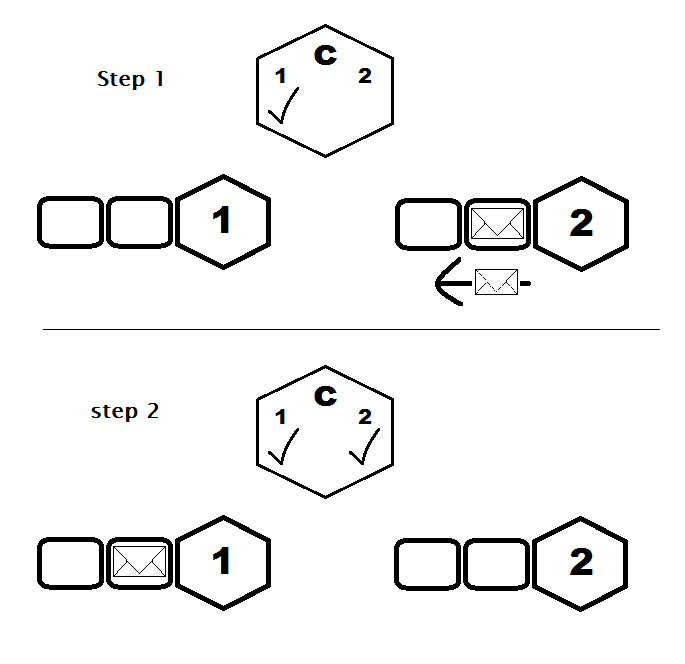
\includegraphics[width=0.7\textwidth]{Analysis/Supercomputing/iterationproblem.png}\label{iterationproblem_img}
\end{figure}

\begin{tabular}{ | p{1cm} | p{6cm} | p{6cm} | }% HAAAAAAAAAAAAAAAAAAAAAAAAAAAX
\hline
Step & Actor 1 & Actor 2 \\\hline
1 & Has no message and is not running, so it sends a message to the controller & Evaluates a message, which causes it to send a message to actor 1 \\\hline
2 & Receives the message from actor 2 and starts running & Has no message and is not running, so it sends a message to the controller \\\hline
\end{tabular}\\

Now the controller will have received all reports, and will proceed with the next iteration, even though actor 1 is still running. Even if actor 1 was to send a message to the controller, revoking the original message, it could arrive too late, which would not give the security wanted by the iteration feature.

During the design of the language, two solutions where considered.

\subsubsection{Pause and Check}

This solution is the direct solution to the naïve approach. It solves the problem through a pause. Whenever the controller has received checks from all actors in the group, it will force an interrupt on the actors. This will allow the controller to go through the actors, directly checking whether their messagebox is empty or they are currently running. This solution however imposes a potential for inefficiency, especially in systems with many actors, which will cause the controller runthrough to become a significant overhead.

\subsubsection{Semaphore}

This solution builds on the idea of a central controlling semaphore shared by the group of actors. Whenever a message is sent, the semaphore is incremented, and whenever a message has been evaluated the semaphore is decremented. Since the increment happens before the decrement, it should effectively only become lower if an actor sent fewer messages than it received. This solution removes the overhead of checking actors, and deals with the problem of the race condition. However it requires a critical region with a semaphore, which could also potentially provide a significant slowdown by bottlenecking actors at the semaphore, even after optimisations are made. This solution was preferred due to the lack of directly halting running actors.

\subsubsection{Delimitation}

For the current project, the implementation of discrete simulations would not be completed due to time constraints. Even so, efforts have been made to ease a future implementation, in order to keep the language true to its goal of supporting both continuous and discrete simulations.
